\documentclass{beamer}


\mode<presentation> {
	\usetheme{PaloAlto}
}

%%
\makeatletter
\setbeamertemplate{subsubsection in sidebar}
  {\vspace*{-\baselineskip}}
\setbeamertemplate{subsubsection in sidebar shaded}
  {\vspace*{-\baselineskip}}
\makeatother
%%

%%
\setbeamertemplate{theorems}[numbered]
%%

\definecolor{Garnet}{RGB}{130,0,20}
\usecolortheme[named=Garnet]{structure}

\logo{\includegraphics[width=1.5cm]{USClogo.png}}

%\setbeamercolor{title}{fg=red!60!black,bg=white!50!black}
%\usecolortheme{beaver}
%\usecolortheme{crane}
\usefonttheme{structuresmallcapsserif}
\usefonttheme[onlysmall]{structurebold}



\usepackage{graphicx}
\usepackage{mathtools}
\usepackage{latexsym}
\usepackage{amsfonts}
\usepackage[only,ninrm,elvrm,twlrm,sixrm,egtrm,tenrm]{rawfonts}
\usepackage{indentfirst}
\usepackage[noend]{algorithmic}
\usepackage{algorithm}
\usepackage{enumerate}
\usepackage{graphicx,psfrag}
\usepackage{epsfig}
%\usepackage[pdflatex]{graphicx}
%\usepackage{epstopdf}
\usepackage{ulem}
\usepackage{animate} %need the animate.sty file
\usepackage{tikz}

\newcommand*{\defeq}{\mathrel{\vcenter{\baselineskip0.5ex \lineskiplimit0pt
                     \hbox{\scriptsize.}\hbox{\scriptsize.}}}%
                     =}
\DeclarePairedDelimiter\ceil{\lceil}{\rceil}
\DeclarePairedDelimiter\floor{\lfloor}{\rfloor}

\input epsf



\usepackage[english]{babel}
% or whatever

\usepackage[latin1]{inputenc}
% or whatever

\usepackage{times}
\usepackage[T1]{fontenc}
% Or whatever. Note that the encoding and the font should match. If T1
% does not look nice, try deleting the line with the fontenc.

\title % (optional, use only with long paper titles)
{Noncommutative Projective Schemes}


\author[Clifton]
{Blake Farman~\inst{1}}

\institute[USC]{
\inst{1}
University of South Carolina, Columbia, SC USA}
%\inst{2}
%East Carolina University, Greenville, NC USA\\
%\inst{3}
%University of Johannesburg, Auckland Park, South Africa}

\date[May 28, 2015]

%\subject{Irredundant and Mixed Ramsey Numbers}
\setbeamercolor{alerted text}{fg=red!60!black}
\setbeamercolor{block title}{bg=white!50!black,fg=red!60!black}

\begin{document}

\begin{frame}
  \titlepage
\end{frame}

\begin{frame}
  \frametitle{Outline}
  \tableofcontents[pausesections]
\end{frame}




\section{Packing Chromatic Number}

\begin{frame}{The Packing Chromatic Number}
\begin{itemize}
\item  Packing colorings were inspired by a frequency assignment problem in broadcasting.
\item This coloring was first introduced by Goddard, Harris, Hedetniemi, Hedetniemi, and Rall (2008) where it was called {\it{broadcast coloring}}.
\item Bre\v sar, Klav\v zar, and Rall (2007) were the first to use the term packing coloring.
\end{itemize}
\end{frame}

\begin{frame}{Definition}
Let $G$ be a simple connected graph of order $n$ and let $i$ be a positive integer.  $X_i\subseteq V(G)$ is called an \alert{{\it{i-packing}}} if vertices in $X_i$ are pairwise distance more than $i$ apart.  A \alert{{\it{packing coloring}}} of $G$ is a partition $X=\{X_1,X_2,X_3,\ldots,X_k \}$ of $V(G)$ such that each color class $X_i$ is an $i$-packing.  The minimum order $k$ of a packing coloring is called the \alert{{\it{packing chromatic number}}} of $G$, denoted by $\chi_{\rho}(G)$.  
\end{frame}

\begin{frame}{Example}
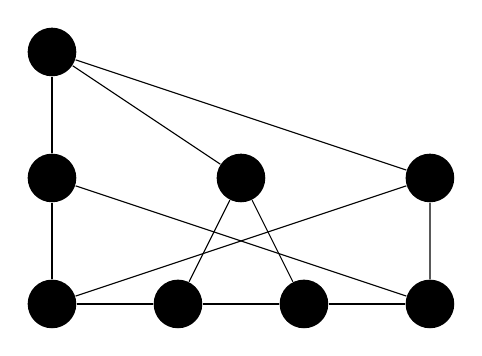
\begin{tikzpicture}
  [scale=.8,auto=center,every node/.style={circle}]
  \node [fill] (n1) at (0,4) {1};
  \node [fill] (n2) at (0,2) {2};
  \node [fill] (n3) at (3,2) {3};
  \node [fill] (n4) at (6,2) {4};
  \node [fill] (n5) at (0,0) {1};
  \node [fill] (n6) at (2,0) {5};
  \node [fill] (n7) at (4,0) {1};
  \node [fill] (n8) at (6,0) {6};

  \foreach \from/\to in {n1/n2,n1/n3,n1/n4,n2/n5,n2/n8,n3/n6,n3/n7,n4/n8,n4/n5,n5/n6,n6/n7,n7/n8}
    \draw (\from) -- (\to);

\end{tikzpicture}
\end{frame}

\begin{frame}{Example}
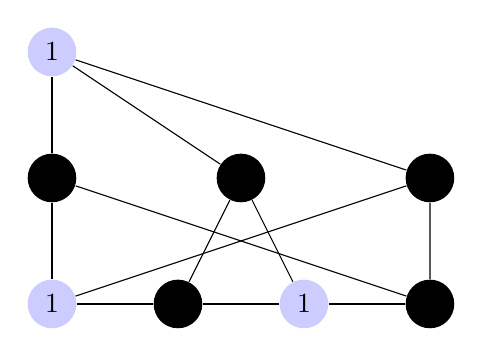
\begin{tikzpicture}
  [scale=.8,auto=center,every node/.style={circle}]
  \node [fill=blue!20] (n1) at (0,4) {1};
  \node [fill] (n2) at (0,2) {2};
  \node [fill] (n3) at (3,2) {3};
  \node [fill] (n4) at (6,2) {4};
  \node [fill=blue!20] (n5) at (0,0) {1};
  \node [fill] (n6) at (2,0) {5};
  \node [fill=blue!20] (n7) at (4,0) {1};
  \node [fill] (n8) at (6,0) {6};

  \foreach \from/\to in {n1/n2,n1/n3,n1/n4,n2/n5,n2/n8,n3/n6,n3/n7,n4/n8,n4/n5,n5/n6,n6/n7,n7/n8}
    \draw (\from) -- (\to);

\end{tikzpicture}
\end{frame}

\begin{frame}{Example}
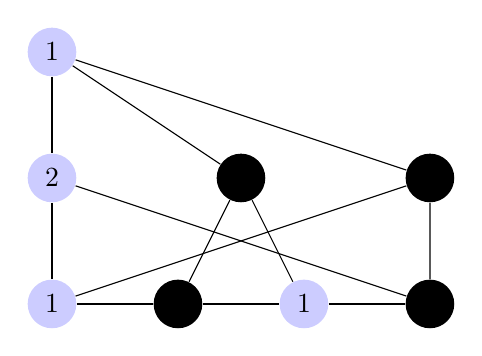
\begin{tikzpicture}
  [scale=.8,auto=center,every node/.style={circle}]
  \node [fill=blue!20] (n1) at (0,4) {1};
  \node [fill=blue!20] (n2) at (0,2) {2};
  \node [fill] (n3) at (3,2) {3};
  \node [fill] (n4) at (6,2) {4};
  \node [fill=blue!20] (n5) at (0,0) {1};
  \node [fill] (n6) at (2,0) {5};
  \node [fill=blue!20] (n7) at (4,0) {1};
  \node [fill] (n8) at (6,0) {6};

  \foreach \from/\to in {n1/n2,n1/n3,n1/n4,n2/n5,n2/n8,n3/n6,n3/n7,n4/n8,n4/n5,n5/n6,n6/n7,n7/n8}
    \draw (\from) -- (\to);

\end{tikzpicture}
\end{frame}

\begin{frame}{Example}
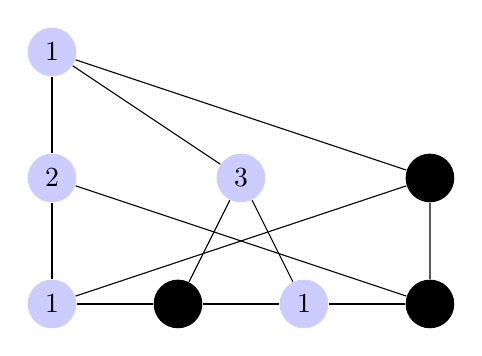
\begin{tikzpicture}
  [scale=.8,auto=center,every node/.style={circle}]
  \node [fill=blue!20] (n1) at (0,4) {1};
  \node [fill=blue!20] (n2) at (0,2) {2};
  \node [fill=blue!20] (n3) at (3,2) {3};
  \node [fill] (n4) at (6,2) {4};
  \node [fill=blue!20] (n5) at (0,0) {1};
  \node [fill] (n6) at (2,0) {5};
  \node [fill=blue!20] (n7) at (4,0) {1};
  \node [fill] (n8) at (6,0) {6};

  \foreach \from/\to in {n1/n2,n1/n3,n1/n4,n2/n5,n2/n8,n3/n6,n3/n7,n4/n8,n4/n5,n5/n6,n6/n7,n7/n8}
    \draw (\from) -- (\to);

\end{tikzpicture}
\end{frame}

\begin{frame}{Example}
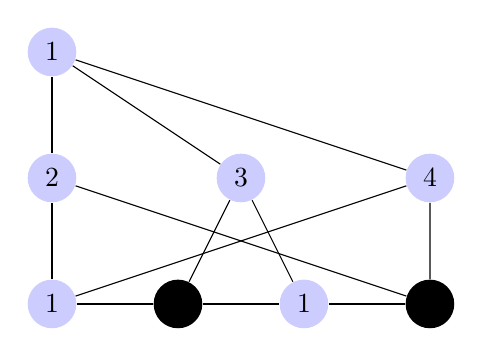
\begin{tikzpicture}
  [scale=.8,auto=center,every node/.style={circle}]
  \node [fill=blue!20] (n1) at (0,4) {1};
  \node [fill=blue!20] (n2) at (0,2) {2};
  \node [fill=blue!20] (n3) at (3,2) {3};
  \node [fill=blue!20] (n4) at (6,2) {4};
  \node [fill=blue!20] (n5) at (0,0) {1};
  \node [fill] (n6) at (2,0) {5};
  \node [fill=blue!20] (n7) at (4,0) {1};
  \node [fill] (n8) at (6,0) {6};

  \foreach \from/\to in {n1/n2,n1/n3,n1/n4,n2/n5,n2/n8,n3/n6,n3/n7,n4/n8,n4/n5,n5/n6,n6/n7,n7/n8}
    \draw (\from) -- (\to);

\end{tikzpicture}
\end{frame}

\begin{frame}{Example}
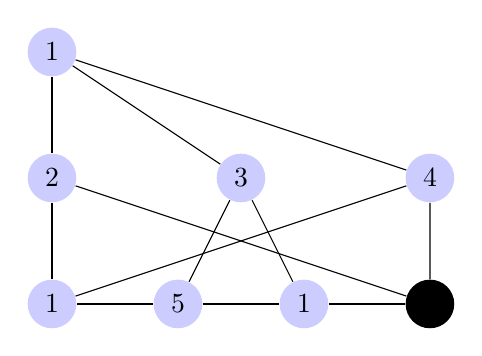
\begin{tikzpicture}
  [scale=.8,auto=center,every node/.style={circle}]
  \node [fill=blue!20] (n1) at (0,4) {1};
  \node [fill=blue!20] (n2) at (0,2) {2};
  \node [fill=blue!20] (n3) at (3,2) {3};
  \node [fill=blue!20] (n4) at (6,2) {4};
  \node [fill=blue!20] (n5) at (0,0) {1};
  \node [fill=blue!20] (n6) at (2,0) {5};
  \node [fill=blue!20] (n7) at (4,0) {1};
  \node [fill] (n8) at (6,0) {6};

  \foreach \from/\to in {n1/n2,n1/n3,n1/n4,n2/n5,n2/n8,n3/n6,n3/n7,n4/n8,n4/n5,n5/n6,n6/n7,n7/n8}
    \draw (\from) -- (\to);

\end{tikzpicture}
\end{frame}


\begin{frame}{Example}
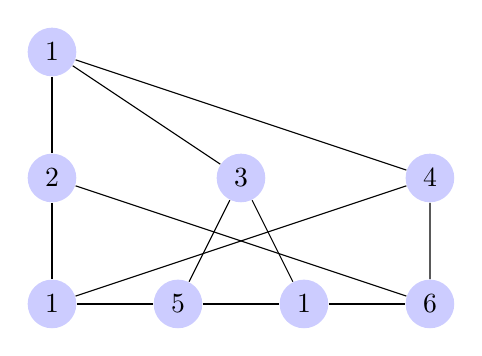
\begin{tikzpicture}
  [scale=.8,auto=center,every node/.style={circle}]
  \node [fill=blue!20] (n1) at (0,4) {1};
  \node [fill=blue!20] (n2) at (0,2) {2};
  \node [fill=blue!20] (n3) at (3,2) {3};
  \node [fill=blue!20] (n4) at (6,2) {4};
  \node [fill=blue!20] (n5) at (0,0) {1};
  \node [fill=blue!20] (n6) at (2,0) {5};
  \node [fill=blue!20] (n7) at (4,0) {1};
  \node [fill=blue!20] (n8) at (6,0) {6};

  \foreach \from/\to in {n1/n2,n1/n3,n1/n4,n2/n5,n2/n8,n3/n6,n3/n7,n4/n8,n4/n5,n5/n6,n6/n7,n7/n8}
    \draw (\from) -- (\to);

\end{tikzpicture}
\end{frame}


\begin{frame}{The Packing Chromatic Number}
\begin{itemize}
\item Goddard et al. (2008) investigated, amongst others, the packing chromatic number of paths, trees, and the infinite square lattice, $\mathbb{Z}^2$.  They found that for the square lattice, $9\leq \chi_{\rho}(\mathbb{Z}^2)\leq 23$.
\item Most recently the bounds have been improved to $12\leq\chi_\rho(\mathbb{Z}^2)\leq 17$.
\item $\chi_{\rho}(G)$ for lattices, trees, and Cartesian products in general was also considered by Bre\v sar et al. (2007) and Finbow and Rall in 2010.
\item C., Hattingh, Jonck examined the lower bound for 3-regular graphs and provide a class of graphs which achieve the bound $\chi_\rho(G)\geq 4$.
\end{itemize}
\end{frame}

\begin{frame}{The Packing Chromatic Number}
\begin{itemize}
\item Goddard et al. (2008) showed that finding $\chi_{\rho}(G)$ for general graphs is NP-complete and deciding whether $\chi_{\rho}(G)\leq 4$ is also NP-complete.
\item Fiala and Golovach (2010) showed that the decision whether a tree allows a packing coloring with at most $k$ classes is NP-complete.
\end{itemize}
\end{frame}

\begin{frame}{Surprise!}
\begin{block}{Theorem (Sloper, 2004):}
The infinite 3-regular tree has packing chromatic number 7.
\end{block}
\end{frame}

\begin{frame}{Eccentric Coloring}
\begin{block}{Definition:}
An \emph{eccentric coloring} of a graph $G=(V,E)$ is a function $color:V\rightarrow\mathbb{N}$ such that
\begin{enumerate}
\item For all $u,v\in V$, $(color(u)=color(v))\Rightarrow d(u,v)>color(u)$
\item For all $v\in V$, $color(v)\leq e(v)$ where $e(v)=\max_{u\in V}\{d(v,u)\}$
\end{enumerate}
\end{block}
\end{frame}

\begin{frame}
\begin{block}{Definition:}
A \emph{binary tree} is a tree where all the vertices have degree 1, 2, or 3.
\end{block}
\pause
\begin{block}{Definition:}
We inductively define a \emph{complete binary tree} $B_i$:
\begin{enumerate}
\item $B_1\defeq 1$ vertex, the root.  This vertex is Level 1.
\item $B_h\defeq$ Start with $B_{h-1}$ and append 2 new leaves to each leaf of $B_{h-1}$.  The new leaves are Level $h$.
\end{enumerate}
The height of a complete binary tree is $h=d(root,leaf)+1$.
\end{block}
\end{frame}

\begin{frame}{Sloper's Theorem}
\begin{block}{Theorem (Sloper, 2004):}
Any complete binary tree of height of three or more is eccentrically colorable with 7 colors or less.
\end{block}
\end{frame}


%INSERT SLOPER CONSTRUCTION
\begin{frame}{Sloper's Construction}

{\bf{Defintion:}} An {\it{expandable eccentric coloring}} of a complete binary tree $T=(V,E)$ is a coloring such that
\begin{itemize}
\item For all $u,v\in V$, (color(u)=color(v))$\Rightarrow d(u,v)>color(u)$
\pause
\item For all $v\in V$, color(v)$\leq$e(v)
\pause
\item The root (level 1) is colored 1
\pause
\item All vertices on odd levels are also colored 1
\pause
\item Every vertex colored 1 has at least one child colored 2 or 3
\pause
\item color(v)=6 and color(u)=7 $\Rightarrow d(u,v)\geq 5$
\pause
\item color(p)$\in\{4,5,6,7\}\Rightarrow$ p's children each have children colored 2 and 3
\pause
\item For all $u\in V$, color(u)$\leq 7$
\end{itemize}
\end{frame}

\begin{frame}{Example}
\begin{figure}[hbt]\centering
\begin{tabular}{c}
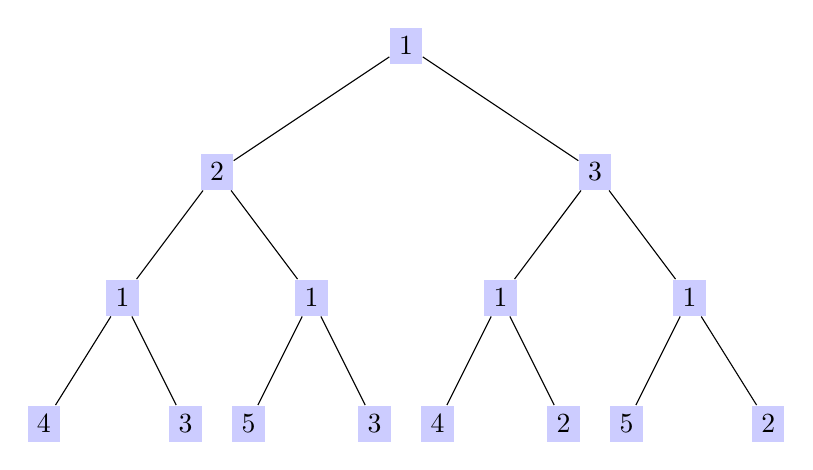
\begin{tikzpicture}[scale=.8]
\node[fill=blue!20] (v1) at (6,8) {1};
\node[fill=blue!20] (v2) at (3,6) {2};
\node[fill=blue!20] (v3) at (9,6) {3};
\node[fill=blue!20] (v4) at (1.5,4) {1};
\node[fill=blue!20] (v5) at (4.5,4) {1};
\node[fill=blue!20] (v6) at (7.5,4) {1};
\node[fill=blue!20] (v7) at (10.5,4) {1};

\node[fill=blue!20] (v8) at (.25,2) {4};
\node[fill=blue!20] (v9) at (2.5,2) {3};
\node[fill=blue!20] (v10) at (3.5,2) {5};
\node[fill=blue!20] (v11) at (5.5,2) {3};
\node[fill=blue!20] (v12) at (6.5,2) {4};
\node[fill=blue!20] (v13) at (8.5,2) {2};
\node[fill=blue!20] (v14) at (9.5,2) {5};
\node[fill=blue!20] (v15) at (11.75,2) {2};
\foreach \from/\to in {v1/v2,v1/v3,v2/v4,v2/v5,v3/v6,v3/v7,v4/v8,v4/v9,v5/v10,v5/v11,v6/v12,v6/v13,v7/v14,v7/v15}
\draw (\from) -- (\to);
\end{tikzpicture}
\end{tabular}
\caption{Expandable eccentric coloring}\label{eccexample}
\end{figure}
\end{frame}

\begin{frame}{The Proof}
\begin{block}{Lemma:}
An expandable eccentric coloring of a complete binary tree of height $n$ can be extended to an expandable eccentric coloring of height $(n+1)$.
\end{block}
{\bfseries{Sketch of Proof:}} Note that we may assume $n$ is odd. Then all vertices at level $n$ are colored 1.  Consider a leaf $u$ at level $n+1$ and its grandparent $p$.  If $color(p)\in\{4,5,6,7\}$ then $u$ and its sibling, say $v$, are assigned the colors 2 and 3 (order does not matter).
\end{frame}

\begin{frame}{$color(p)\in\{4,5,6,7\}$}
\begin{figure}[hbt]\centering
\begin{center}
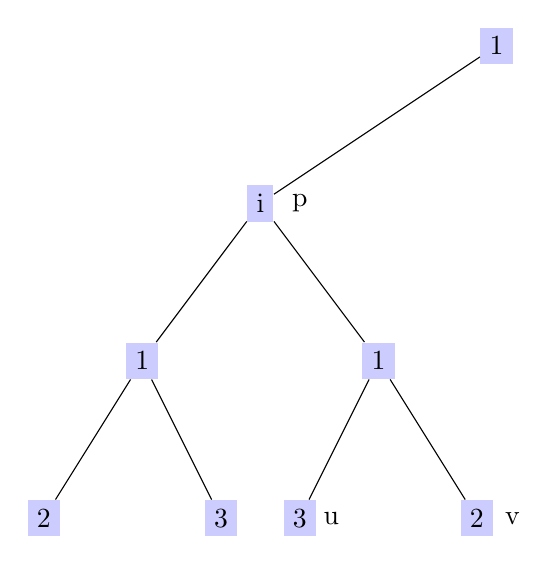
\begin{tikzpicture}
[scale=1]
\node[fill=blue!20] (v1) at (6,8) {1};
\node[fill=blue!20] (v2) at (3,6) {i};
\node[fill=blue!20] (v4) at (1.5,4) {1};
\node[fill=blue!20] (v5) at (4.5,4) {1};
\node[fill=blue!20] (v8) at (.25,2) {2};
\node[fill=blue!20] (v9) at (2.5,2) {3};
\node[fill=blue!20] (v10) at (3.5,2) {3};
\node[fill=blue!20] (v11) at (5.75,2) {2};
\node (v12) at (3.5,6) {p};
\node (v13) at (3.9,2) {u};
\node (v14) at (6.2,2) {v};
\foreach \from/\to in {v1/v2,v2/v4,v2/v5,v4/v8,v4/v9,v5/v10,v5/v11}
\draw (\from) -- (\to);
\end{tikzpicture}
\end{center}
\caption{A coloring of level $n+1$ if $color(p)\in\{4,5,6,7\}$}\label{colorpknown}
\end{figure}
\end{frame}

\begin{frame}{The Proof (cont.)}
We now consider the case when $color(p)=2$ (the case when $color(p)=3$ is handled similarly).\\ \pause
Since for any grandchild $j$ of $p$, $d(j,p)=2$, we have $color(j)\neq 2$.\\ \pause  Let $u,v,w,z$ be $p$'s grandchildren with pairs of siblings $\{u,v\}$ and $\{w,z\}$.  We consider all vertices at distance at most 6 from $u,v,w,$ and $z$ (any vertex at distance 7 from $u,v,w,$ or $z$ must be on an odd level and is already colored 1).  By rule 5, two of $p$'s grandchildren (which are not siblings) must receive the color 3.  Without loss of generality suppose $color(v)=color(z)=3$.
\end{frame}

\begin{frame}{$color(p)=2$}
\begin{figure}
\begin{center}
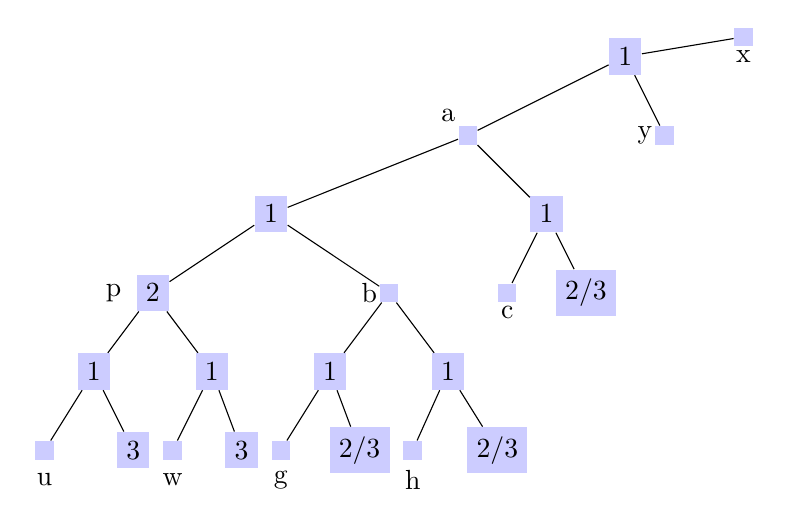
\begin{tikzpicture}
[scale=.5]
\node[fill=blue!20] (v1) at (6,8) {1};
\node[fill=blue!20] (v2) at (3,6) {2};
\node (v16) at (2,6) {p};
\node[fill=blue!20] (v3) at (9,6) {};
\node (v28) at (8.5,6) {b};

\node[fill=blue!20] (v4) at (1.5,4) {1};
\node[fill=blue!20] (v5) at (4.5,4) {1};
\node[fill=blue!20] (v6) at (7.5,4) {1};
\node[fill=blue!20] (v7) at (10.5,4) {1};

\node[fill=blue!20] (v8) at (.25,2) {};
\node (v33) at (.25,1.25) {u};
\node[fill=blue!20] (v9) at (2.5,2) {3};

\node[fill=blue!20] (v10) at (3.5,2) {};
\node (v34) at (3.5,1.25) {w};
\node[fill=blue!20] (v11) at (5.25,2) {3};

\node[fill=blue!20] (v12) at (6.25,2) {};
\node (v26) at (6.25,1.25) {g};
\node[fill=blue!20] (v13) at (8.25,2) {2/3};
\node[fill=blue!20] (v14) at (9.6,2) {};
\node (v27) at (9.6,1.25) {h};
\node[fill=blue!20] (v15) at (11.75,2) {2/3};

\node[fill=blue!20] (v19) at (11,10) {};
\node (v29) at (10.5,10.5) {a};
\node[fill=blue!20] (v20) at (13,8) {1};
\node[fill=blue!20] (v21) at (12,6) {};
\node (v30) at (12,5.5) {c};
\node[fill=blue!20] (v22) at (14,6) {2/3};

\node[fill=blue!20] (v23) at (15,12) {1};
\node[fill=blue!20] (v25) at (16,10) {};
\node (v31) at (15.5,10) {y};
\node[fill=blue!20] (v24) at (18,12.5) {};
\node (v32) at (18,12) {x};

\foreach \from/\to in {v1/v2,v1/v3,v2/v4,v2/v5,v3/v6,v3/v7,v4/v8,v4/v9,v5/v10,v5/v11,v6/v12,v6/v13,v7/v14,v7/v15,v1/v19,v19/v23,v19/v20,v20/v21,v20/v22,v23/v24,v23/v25}
\draw (\from) -- (\to);
\end{tikzpicture}
\end{center}
\caption{The subtree examined when $color(p)=2$}\label{subtree}
\end{figure}
\end{frame}

\begin{frame}{$color(p)=2$ and $color(a)=3$}
\begin{figure}
\begin{center}
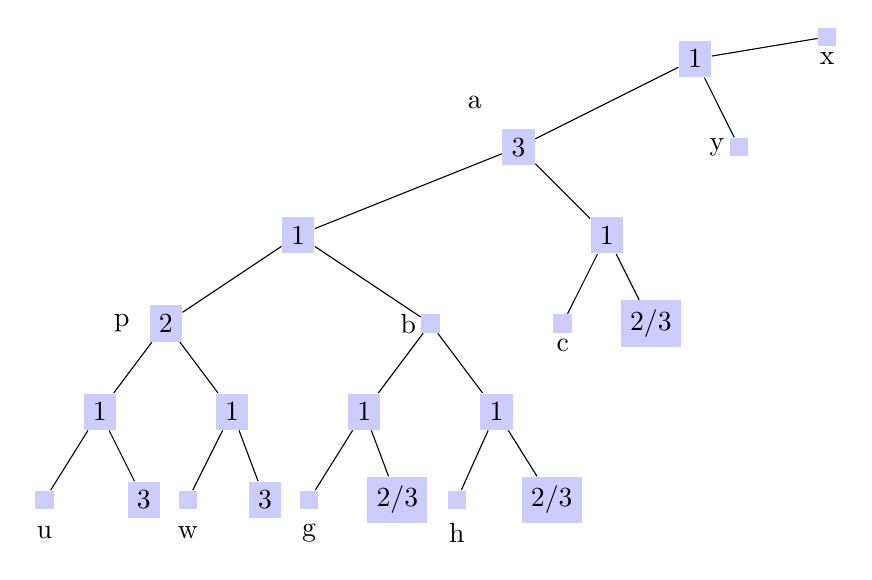
\begin{tikzpicture}
[scale=.56]
\node[fill=blue!20] (v1) at (6,8) {1};
\node[fill=blue!20] (v2) at (3,6) {2};
\node (v16) at (2,6) {p};
\node[fill=blue!20] (v3) at (9,6) {};
\node (v28) at (8.5,6) {b};

\node[fill=blue!20] (v4) at (1.5,4) {1};
\node[fill=blue!20] (v5) at (4.5,4) {1};
\node[fill=blue!20] (v6) at (7.5,4) {1};
\node[fill=blue!20] (v7) at (10.5,4) {1};

\node[fill=blue!20] (v8) at (.25,2) {};
\node (v33) at (.25,1.25) {u};
\node[fill=blue!20] (v9) at (2.5,2) {3};

\node[fill=blue!20] (v10) at (3.5,2) {};
\node (v34) at (3.5,1.25) {w};
\node[fill=blue!20] (v11) at (5.25,2) {3};

\node[fill=blue!20] (v12) at (6.25,2) {};
\node (v26) at (6.25,1.25) {g};
\node[fill=blue!20] (v13) at (8.25,2) {2/3};
\node[fill=blue!20] (v14) at (9.6,2) {};
\node (v27) at (9.6,1.25) {h};
\node[fill=blue!20] (v15) at (11.75,2) {2/3};

\node[fill=blue!20] (v19) at (11,10) {3};
\node (v29) at (10,11) {a};
\node[fill=blue!20] (v20) at (13,8) {1};
\node[fill=blue!20] (v21) at (12,6) {};
\node (v30) at (12,5.5) {c};
\node[fill=blue!20] (v22) at (14,6) {2/3};

\node[fill=blue!20] (v23) at (15,12) {1};
\node[fill=blue!20] (v25) at (16,10) {};
\node (v31) at (15.5,10) {y};
\node[fill=blue!20] (v24) at (18,12.5) {};
\node (v32) at (18,12) {x};

\foreach \from/\to in {v1/v2,v1/v3,v2/v4,v2/v5,v3/v6,v3/v7,v4/v8,v4/v9,v5/v10,v5/v11,v6/v12,v6/v13,v7/v14,v7/v15,v1/v19,v19/v23,v19/v20,v20/v21,v20/v22,v23/v24,v23/v25}
\draw (\from) -- (\to);
\end{tikzpicture}
\end{center}
\end{figure}
\end{frame}


\begin{frame}{$color(p)=2$ and $color(a)=3$}
\begin{figure}
\begin{center}
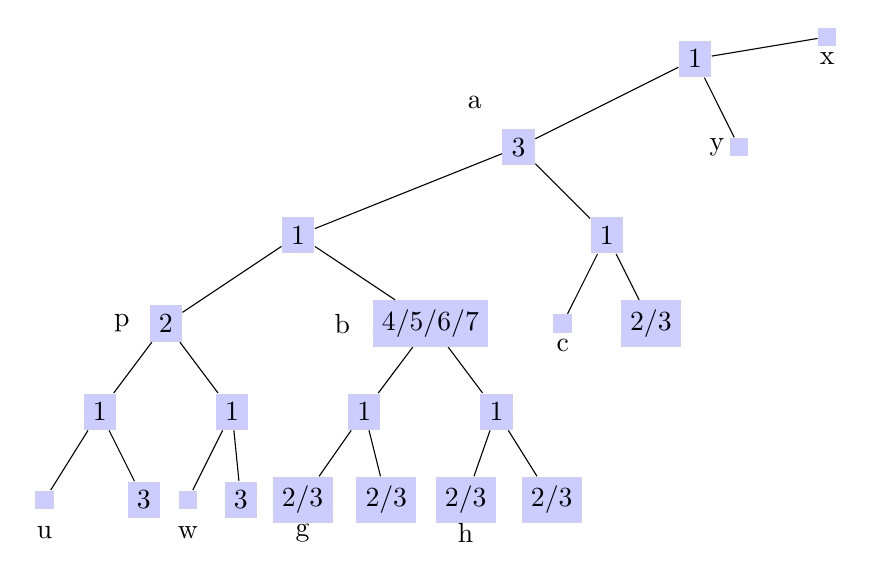
\begin{tikzpicture}
[scale=.56]
\node[fill=blue!20] (v1) at (6,8) {1};
\node[fill=blue!20] (v2) at (3,6) {2};
\node (v16) at (2,6) {p};
\node[fill=blue!20] (v3) at (9,6) {4/5/6/7};
\node (v28) at (7,6) {b};

\node[fill=blue!20] (v4) at (1.5,4) {1};
\node[fill=blue!20] (v5) at (4.5,4) {1};
\node[fill=blue!20] (v6) at (7.5,4) {1};
\node[fill=blue!20] (v7) at (10.5,4) {1};

\node[fill=blue!20] (v8) at (.25,2) {};
\node (v33) at (.25,1.25) {u};
\node[fill=blue!20] (v9) at (2.5,2) {3};

\node[fill=blue!20] (v10) at (3.5,2) {};
\node (v34) at (3.5,1.25) {w};
\node[fill=blue!20] (v11) at (4.7,2) {3};

\node[fill=blue!20] (v12) at (6.1,2) {2/3};
\node (v26) at (6.1,1.25) {g};
\node[fill=blue!20] (v13) at (8.,2) {2/3};
\node[fill=blue!20] (v14) at (9.8,2) {2/3};
\node (v27) at (9.8,1.25) {h};
\node[fill=blue!20] (v15) at (11.75,2) {2/3};

\node[fill=blue!20] (v19) at (11,10) {3};
\node (v29) at (10,11) {a};
\node[fill=blue!20] (v20) at (13,8) {1};
\node[fill=blue!20] (v21) at (12,6) {};
\node (v30) at (12,5.5) {c};
\node[fill=blue!20] (v22) at (14,6) {2/3};

\node[fill=blue!20] (v23) at (15,12) {1};
\node[fill=blue!20] (v25) at (16,10) {};
\node (v31) at (15.5,10) {y};
\node[fill=blue!20] (v24) at (18,12.5) {};
\node (v32) at (18,12) {x};

\foreach \from/\to in {v1/v2,v1/v3,v2/v4,v2/v5,v3/v6,v3/v7,v4/v8,v4/v9,v5/v10,v5/v11,v6/v12,v6/v13,v7/v14,v7/v15,v1/v19,v19/v23,v19/v20,v20/v21,v20/v22,v23/v24,v23/v25}
\draw (\from) -- (\to);
\end{tikzpicture}
\end{center}
\end{figure}
\end{frame}

\begin{frame}{$color(p)=2$ and $color(a)\in\{4,5\}$}
\begin{figure}
\begin{center}
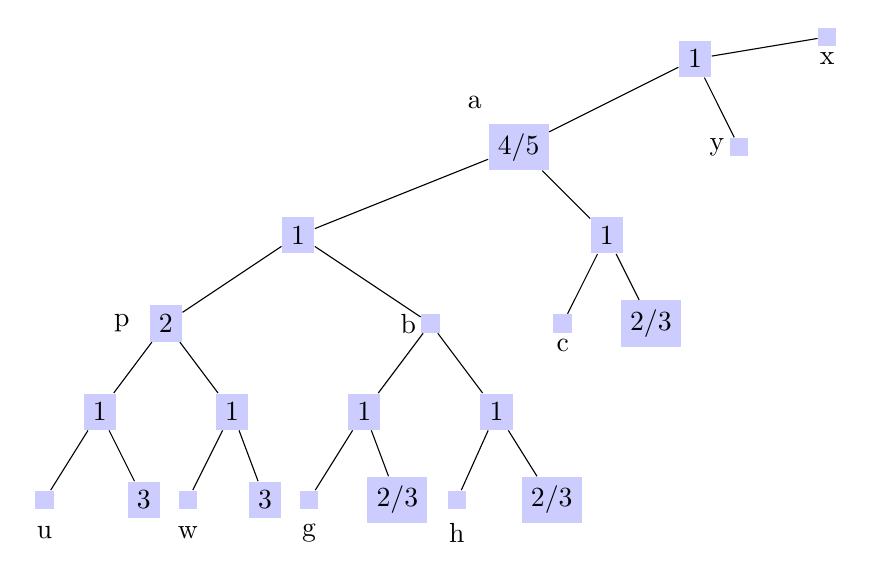
\begin{tikzpicture}
[scale=.56]
\node[fill=blue!20] (v1) at (6,8) {1};
\node[fill=blue!20] (v2) at (3,6) {2};
\node (v16) at (2,6) {p};
\node[fill=blue!20] (v3) at (9,6) {};
\node (v28) at (8.5,6) {b};

\node[fill=blue!20] (v4) at (1.5,4) {1};
\node[fill=blue!20] (v5) at (4.5,4) {1};
\node[fill=blue!20] (v6) at (7.5,4) {1};
\node[fill=blue!20] (v7) at (10.5,4) {1};

\node[fill=blue!20] (v8) at (.25,2) {};
\node (v33) at (.25,1.25) {u};
\node[fill=blue!20] (v9) at (2.5,2) {3};

\node[fill=blue!20] (v10) at (3.5,2) {};
\node (v34) at (3.5,1.25) {w};
\node[fill=blue!20] (v11) at (5.25,2) {3};

\node[fill=blue!20] (v12) at (6.25,2) {};
\node (v26) at (6.25,1.25) {g};
\node[fill=blue!20] (v13) at (8.25,2) {2/3};
\node[fill=blue!20] (v14) at (9.6,2) {};
\node (v27) at (9.6,1.25) {h};
\node[fill=blue!20] (v15) at (11.75,2) {2/3};

\node[fill=blue!20] (v19) at (11,10) {4/5};
\node (v29) at (10,11) {a};
\node[fill=blue!20] (v20) at (13,8) {1};
\node[fill=blue!20] (v21) at (12,6) {};
\node (v30) at (12,5.5) {c};
\node[fill=blue!20] (v22) at (14,6) {2/3};

\node[fill=blue!20] (v23) at (15,12) {1};
\node[fill=blue!20] (v25) at (16,10) {};
\node (v31) at (15.5,10) {y};
\node[fill=blue!20] (v24) at (18,12.5) {};
\node (v32) at (18,12) {x};

\foreach \from/\to in {v1/v2,v1/v3,v2/v4,v2/v5,v3/v6,v3/v7,v4/v8,v4/v9,v5/v10,v5/v11,v6/v12,v6/v13,v7/v14,v7/v15,v1/v19,v19/v23,v19/v20,v20/v21,v20/v22,v23/v24,v23/v25}
\draw (\from) -- (\to);
\end{tikzpicture}
\end{center}
\end{figure}
\end{frame}

\begin{frame}{$color(p)=2$ and $color(a)\in\{4,5\}$}
\begin{figure}
\begin{center}
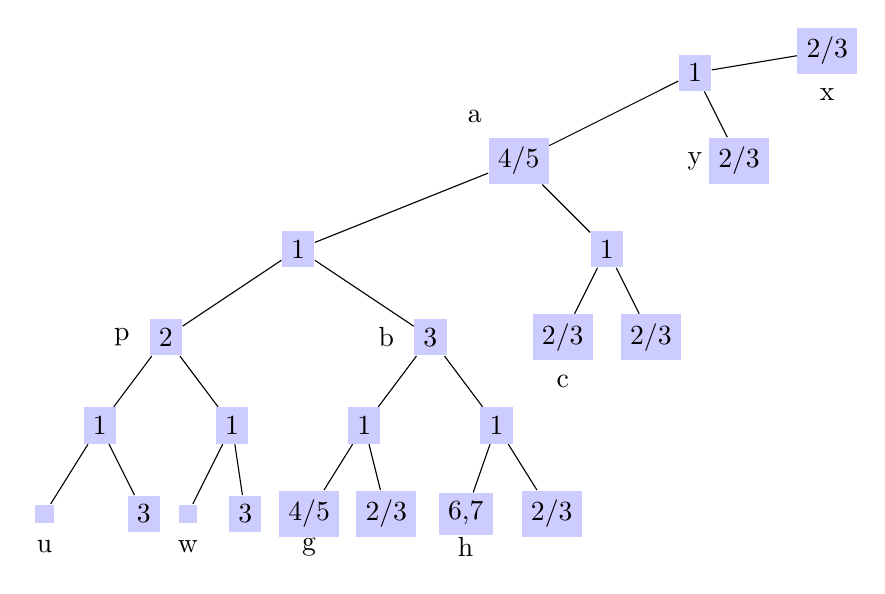
\begin{tikzpicture}
[scale=.56]
\node[fill=blue!20] (v1) at (6,8) {1};
\node[fill=blue!20] (v2) at (3,6) {2};
\node (v16) at (2,6) {p};
\node[fill=blue!20] (v3) at (9,6) {3};
\node (v28) at (8,6) {b};

\node[fill=blue!20] (v4) at (1.5,4) {1};
\node[fill=blue!20] (v5) at (4.5,4) {1};
\node[fill=blue!20] (v6) at (7.5,4) {1};
\node[fill=blue!20] (v7) at (10.5,4) {1};

\node[fill=blue!20] (v8) at (.25,2) {};
\node (v33) at (.25,1.25) {u};
\node[fill=blue!20] (v9) at (2.5,2) {3};

\node[fill=blue!20] (v10) at (3.5,2) {};
\node (v34) at (3.5,1.25) {w};
\node[fill=blue!20] (v11) at (4.8,2) {3};

\node[fill=blue!20] (v12) at (6.25,2) {4/5};
\node (v26) at (6.25,1.25) {g};
\node[fill=blue!20] (v13) at (8,2) {2/3};
\node[fill=blue!20] (v14) at (9.8,2) {6,7};
\node (v27) at (9.8,1.25) {h};
\node[fill=blue!20] (v15) at (11.75,2) {2/3};

\node[fill=blue!20] (v19) at (11,10) {4/5};
\node (v29) at (10,11) {a};
\node[fill=blue!20] (v20) at (13,8) {1};
\node[fill=blue!20] (v21) at (12,6) {2/3};
\node (v30) at (12,5) {c};
\node[fill=blue!20] (v22) at (14,6) {2/3};

\node[fill=blue!20] (v23) at (15,12) {1};
\node[fill=blue!20] (v25) at (16,10) {2/3};
\node (v31) at (15,10) {y};
\node[fill=blue!20] (v24) at (18,12.5) {2/3};
\node (v32) at (18,11.5) {x};

\foreach \from/\to in {v1/v2,v1/v3,v2/v4,v2/v5,v3/v6,v3/v7,v4/v8,v4/v9,v5/v10,v5/v11,v6/v12,v6/v13,v7/v14,v7/v15,v1/v19,v19/v23,v19/v20,v20/v21,v20/v22,v23/v24,v23/v25}
\draw (\from) -- (\to);
\end{tikzpicture}
\end{center}
\end{figure}
\end{frame}

\begin{frame}{$color(p)=2$ and $color(a)\in\{6,7\}$}
\begin{figure}
\begin{center}
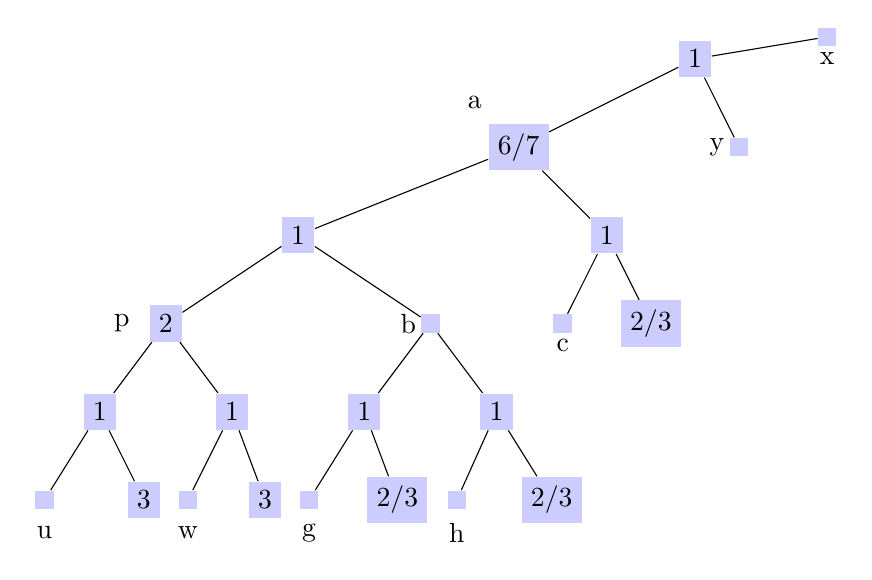
\begin{tikzpicture}
[scale=.56]
\node[fill=blue!20] (v1) at (6,8) {1};
\node[fill=blue!20] (v2) at (3,6) {2};
\node (v16) at (2,6) {p};
\node[fill=blue!20] (v3) at (9,6) {};
\node (v28) at (8.5,6) {b};

\node[fill=blue!20] (v4) at (1.5,4) {1};
\node[fill=blue!20] (v5) at (4.5,4) {1};
\node[fill=blue!20] (v6) at (7.5,4) {1};
\node[fill=blue!20] (v7) at (10.5,4) {1};

\node[fill=blue!20] (v8) at (.25,2) {};
\node (v33) at (.25,1.25) {u};
\node[fill=blue!20] (v9) at (2.5,2) {3};

\node[fill=blue!20] (v10) at (3.5,2) {};
\node (v34) at (3.5,1.25) {w};
\node[fill=blue!20] (v11) at (5.25,2) {3};

\node[fill=blue!20] (v12) at (6.25,2) {};
\node (v26) at (6.25,1.25) {g};
\node[fill=blue!20] (v13) at (8.25,2) {2/3};
\node[fill=blue!20] (v14) at (9.6,2) {};
\node (v27) at (9.6,1.25) {h};
\node[fill=blue!20] (v15) at (11.75,2) {2/3};

\node[fill=blue!20] (v19) at (11,10) {6/7};
\node (v29) at (10,11) {a};
\node[fill=blue!20] (v20) at (13,8) {1};
\node[fill=blue!20] (v21) at (12,6) {};
\node (v30) at (12,5.5) {c};
\node[fill=blue!20] (v22) at (14,6) {2/3};

\node[fill=blue!20] (v23) at (15,12) {1};
\node[fill=blue!20] (v25) at (16,10) {};
\node (v31) at (15.5,10) {y};
\node[fill=blue!20] (v24) at (18,12.5) {};
\node (v32) at (18,12) {x};

\foreach \from/\to in {v1/v2,v1/v3,v2/v4,v2/v5,v3/v6,v3/v7,v4/v8,v4/v9,v5/v10,v5/v11,v6/v12,v6/v13,v7/v14,v7/v15,v1/v19,v19/v23,v19/v20,v20/v21,v20/v22,v23/v24,v23/v25}
\draw (\from) -- (\to);
\end{tikzpicture}
\end{center}
\end{figure}
\end{frame}

\begin{frame}{$color(p)=2$ and $color(a)\in\{6,7\}$}
\begin{figure}
\begin{center}
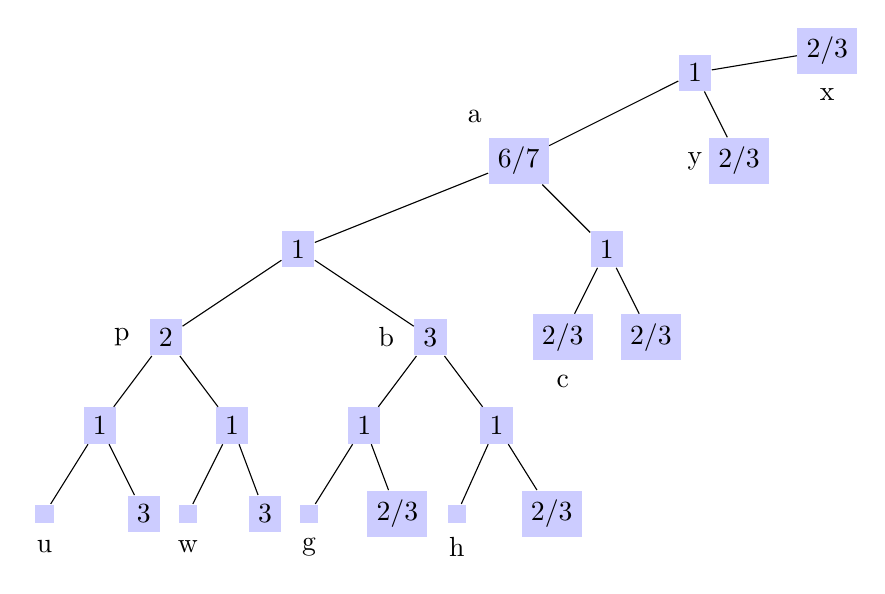
\begin{tikzpicture}
[scale=.56]
\node[fill=blue!20] (v1) at (6,8) {1};
\node[fill=blue!20] (v2) at (3,6) {2};
\node (v16) at (2,6) {p};
\node[fill=blue!20] (v3) at (9,6) {3};
\node (v28) at (8,6) {b};

\node[fill=blue!20] (v4) at (1.5,4) {1};
\node[fill=blue!20] (v5) at (4.5,4) {1};
\node[fill=blue!20] (v6) at (7.5,4) {1};
\node[fill=blue!20] (v7) at (10.5,4) {1};

\node[fill=blue!20] (v8) at (.25,2) {};
\node (v33) at (.25,1.25) {u};
\node[fill=blue!20] (v9) at (2.5,2) {3};

\node[fill=blue!20] (v10) at (3.5,2) {};
\node (v34) at (3.5,1.25) {w};
\node[fill=blue!20] (v11) at (5.25,2) {3};

\node[fill=blue!20] (v12) at (6.25,2) {};
\node (v26) at (6.25,1.25) {g};
\node[fill=blue!20] (v13) at (8.25,2) {2/3};
\node[fill=blue!20] (v14) at (9.6,2) {};
\node (v27) at (9.6,1.25) {h};
\node[fill=blue!20] (v15) at (11.75,2) {2/3};

\node[fill=blue!20] (v19) at (11,10) {6/7};
\node (v29) at (10,11) {a};
\node[fill=blue!20] (v20) at (13,8) {1};
\node[fill=blue!20] (v21) at (12,6) {2/3};
\node (v30) at (12,5) {c};
\node[fill=blue!20] (v22) at (14,6) {2/3};

\node[fill=blue!20] (v23) at (15,12) {1};
\node[fill=blue!20] (v25) at (16,10) {2/3};
\node (v31) at (15,10) {y};
\node[fill=blue!20] (v24) at (18,12.5) {2/3};
\node (v32) at (18,11.5) {x};

\foreach \from/\to in {v1/v2,v1/v3,v2/v4,v2/v5,v3/v6,v3/v7,v4/v8,v4/v9,v5/v10,v5/v11,v6/v12,v6/v13,v7/v14,v7/v15,v1/v19,v19/v23,v19/v20,v20/v21,v20/v22,v23/v24,v23/v25}
\draw (\from) -- (\to);
\end{tikzpicture}
\end{center}
\end{figure}
\end{frame}

\begin{frame}{Surprise!}
Sloper's theorem can not be extended to {\itshape{complete k-ary trees}} with $k\geq 3$!\pause
\begin{block}{Definition:}
 A $k$-ary tree is a tree $T$ such that for all $v\in V(T)$, $d_T(v)\leq k+1$. We can inductively define the complete $k$-ary tree, $T_i$:\\
\begin{enumerate}
\item $T_1\defeq 1$ vertex, the root
\item $T_i\defeq$ Start with $T_{i-1}$ and append $k$ new leaves to each leaf of $T_{i-1}$.
\end{enumerate}
The \emph{height} of a complete $k$-ary tree is $h=d(root,leaf)+1$.
\end{block}
\pause
\begin{block}{Theorem (Sloper, 2004):}
No complete $k$-ary tree, $k\geq 3$, of height $h$, $h\geq 4$ is eccentrically broadcast-colorable.
\end{block}
\end{frame}


\section{d-Regular Graphs}

\begin{frame}{$d$-regular Graphs}
\begin{block}{Theorem (C., Griggs, Lu $2015^{+}$)}
Let $G$ be a $d$-regular graph with girth $g$.  If $d\geq 4$, then $\chi_\rho(G)\geq g-1$.
\end{block}\pause
{\bf{Proof:}} Let $k=g-2$ and assume $\chi_\rho(G)\leq k$.  Then there is a partition $V=V_1\cup V_2\cup\dots\cup V_k$ such that for any $1\leq i\leq k$, and two distinct vertices $u,v\in V_i$, $d(u,v)\geq i$.  For any vertex $u$, let $N_i(u)$ be the set of vertices of distance at most $i$ from $u$.  Similarly, for any edge $uv$, let $N_i(uv)$ be the set of vertices of distance at most $i$ from $u$ or $v$.  

Note that the induced graph on $N_i(u)$ (for $1\leq i\leq \lfloor\frac{k}{2}\rfloor$) is a tree depending only on $i$.  Similarly, the induced graph of $G$ on $N_i(uv)$ (for $i=1,\dots,\lfloor\frac{k}{2}\rfloor-1$) is a tree depending on $i$.
\end{frame}


\begin{frame}{$d$-regular Graphs}
Thus, $$\vert N_i(u)\vert=1+d+d(d-1)+\dots+d(d-1)^{i-1}=\frac{d(d-1)^i-2}{d-2}$$ and $$\vert N_i(uv)\vert =2(1+(d-1)+\dots+(d-1)^{i-1})=\frac{2d(d-1)^i-2}{d-2}.$$
\end{frame}

\begin{frame}{$d$-regular Graphs}
Now, observe that $\vert V_{2i}\cap N_i(u)\vert\leq 1$ for $i=1,2,\dots,\lfloor\frac{k}{2}\rfloor$ and $\vert V_{2i-1}\cap N_{i-1}(uv)\vert\leq 1$ for $i=1,2,\dots,\lceil\frac{k}{2}\rceil$.  

Thus,
\begin{equation*}
\vert V_{2i}\vert\leq\frac{n}{\vert N_i(u)\vert}=\frac{n(d-2)}{d(d-1)^i-2}{\text{\hspace{.2in}for\hspace{.2in}}}1\leq i\leq\floor*{\frac{k}{2}}
\end{equation*}
and
\begin{equation*}
\vert V_{2i-1}\vert\leq\frac{n}{\vert N_i(uv)\vert}=\frac{n(d-2)}{2d(d-1)^i-2}{\text{\hspace{.2in}for\hspace{.2in}}}1\leq i\leq\ceil*{\frac{k}{2}}.
\end{equation*}
\end{frame}

\begin{frame}{$d$-regular Graphs}
As the series $\phi_i(d)\defeq\sum_{i=1}^{\infty}\frac{d-2}{d(d-1)^i-2}$ and $\nu_i(d)\defeq\sum_{i=1}^{\infty}\frac{d-2}{2d(d-1)^i-2}$ converge and are decreasing functions of $d$, we have
\begin{eqnarray*}
n&=&\sum_{i=1}^k\vert V_i\vert\\
&=&\sum_{i=1}^{\lceil\frac{k}{2}\rceil}\vert V_{2i-1}\vert+\sum_{i=1}^{\lfloor\frac{k}{2}\rfloor}\vert V_{2i}\vert\\
&\leq&\sum_{i=1}^{\lceil\frac{k}{2}\rceil}\frac{n(d-2)}{2d(d-1)^i-2}+\sum_{i=1}^{\lfloor\frac{k}{2}\rfloor}\frac{n(d-2)}{d(d-1)^i-2}\\
&<&n(\phi_i(d)+\nu_i(d))\\
&<&n.
\end{eqnarray*}
\end{frame}


\section{Random Graphs}

\begin{frame}{Random Graphs}
\begin{itemize}
\item Erd\H{o}s and R\'{e}nyi are given credit for first implementing the use of random graphs in probabilistic proofs of the existence of graphs with special properties such as arbitrarily large girth and chromatic number.
\item The first combinatorial structures to be studied probabilistically were tournaments.
\item Applications of random graphs are found in all areas in which complex networks need to be modeled.
\end{itemize}
\end{frame}

\begin{frame}{Configuration Model}
Let $\mathcal{G}_{n,d}$ denote the uniform probability space of $d$-regular graphs on the $n$ vertices $\{1,2,\dots,n\}$ where $dn$ is even.  Consider a set of $dn$ points partitioned into $n$ subsets $v_1,v_2,\dots,v_n$ of $d$ points each.  Apply a perfect matching of the points into $\frac{1}{2}dn$ pairs.  A pairing corresponds to a multigraph in which the subsets are the vertices and the pairs are edges.
\end{frame}

\begin{frame}{Configuration Model}
\begin{figure}[hbt]
\includegraphics[scale=.7]{config1.png}
\end{figure}
\end{frame}

\begin{frame}{Configuration Model}
\begin{figure}[hbt]
\includegraphics[scale=.8]{config2.png}
\end{figure}
\end{frame}

\begin{frame}{Configuration Model}
\begin{figure}[hbt]
\includegraphics[scale=.8]{config3.png}
\end{figure}
\end{frame}

\begin{frame}{Configuration Model}
\begin{figure}[hbt]
\includegraphics[scale=.8]{config4.png}
\end{figure}
\end{frame}

\begin{frame}{Configuration Model}
\begin{figure}[hbt]
\includegraphics[scale=.8]{config5.png}
\end{figure}
\end{frame}

\begin{frame}{Configuration Model}
\begin{figure}[hbt]
\includegraphics[scale=.8]{config6.png}
\end{figure}
\end{frame}

\begin{frame}{Configuration Model}
\begin{itemize}
\item The configuration model was first given by Bollob\'as in 1979.
\item Bender and Canfield (1978) show that the probability that $G_{n,d}$ is simple is $(1+o(1))\exp(\frac{1-d^2}{4})$.
\item Let $D$ be the diameter of $G_{n,d}$.  Bollob\'as and de la Vega (1982) showed that with high probability $D=(1+o(1))\log_{d-1}(n)$.
\end{itemize}
\end{frame}

\section{Main Result}

\begin{frame}{Main Result}
\begin{block}{Theorem (C., Griggs, Lu $2015^+$):}
For any integer $d\geq 4$, there exists a positive constant $c_d$ such that $${\bf{P}}(\chi_\rho(G_{n,d})\geq c_dn)=1-o_n(1).$$
\end{block}
\end{frame}


\begin{frame}{Proof}
\begin{block}{Lemma 1}
Let $u$ be a vertex of $G_{n,d}$ and let $N_i(u)$ denote the set of vertices of distance at most $i$ from $u$ in $G_{n,d}$ where $1\leq i\leq (1+o(1))D/2$, where $D$ is the diameter of $G_{n,d}$.  With probability 1-o(1), for all $u$, $\vert N_i(u)\vert\in\{f_i(d),f_i(d)-1\}.$
\end{block}

\begin{block}{Lemma 2}
Let $uv$ be an edge of $G_{n,d}$ and let $N_i(uv)$ denote the set of vertices of distance at most $i$ from $u$ or $v$ in $G_{n,d}$, where $1\leq i\leq (1+o(1))D/2$.  With probability $1-o(1)$, for all $u,v$, $\vert N_i(uv)\vert\in\{g_i(d),g_i(d)-1\}$.
\end{block}
\end{frame}

\begin{frame}{Proof}
\begin{block}{Lemma 3}
Let $u$ be a vertex of $G_{n,d}$ and let $N_i(u)$ denote the set of vertices of distance at most $i$ from $u$ in $G_{n,d}$ where $(1+o(1))D/2\leq i\leq 3D/4$.  With probability 1-o(1), for all $u$, $\frac{f_i(d)}{2}\leq\vert N_i(u)\vert\leq f_i(d).$
\end{block}
\begin{block}{Lemma 4}
Let $uv$ be an edge of $G_{n,d}$ and let $N_i(uv)$ denote the set of vertices of distance at most $i$ from $u$ or $v$ in $G_{n,d}$, where $(1+o(1))D/2\leq i\leq 3D/4$.  With probability $1-o(1)$, for all $u,v$, $\frac{g_i(d)}{2}\leq\vert N_i(uv)\vert\leq g_i(d)$.
\end{block}
\end{frame}

\begin{frame}{Proof}
Finally, we must consider the case when $i\in[3D/4+1, D]$.  Define $G^i=(V,E^i)$ where $E^i=\{(u,v): d(u,v)\leq i{\text{  in  }}G\}$.

Note that as $\alpha(G_{n,d}^i)\leq\alpha(G_{n,d}^j)$ for $i\geq j$, where $\alpha$ is the independence number, we have that $\vert V_i\vert\leq\alpha(G_{n,d}^{i})\leq\alpha(G_{n,d}^j)\leq\frac{2}{f_i(d)}n$ for $i\geq j$.  Thus, $\sum_{i=3/4D}^{D}\vert V_i\vert\leq\sum_{j=(1+o(1))D/2}^{3/4D}\frac{2}{f_j(d)}n<\frac{\epsilon}{6}n.$
\end{frame}

\begin{frame}
\begin{center}
Thank you!
\end{center}
\end{frame}






\end{document}
